\documentclass[xetex,mathserif,serif]{beamer}
\usepackage{polyglossia}
\setdefaultlanguage[babelshorthands=true]{russian}
\usepackage{minted}
\usepackage{tabu}

\useoutertheme{infolines}

\usepackage{fontspec}
\setmainfont{FreeSans}
\newfontfamily{\russianfonttt}{FreeSans}

\tabulinesep=0.7mm

\title{Паттерны, детали реализации}
\author[Юрий Литвинов]{Юрий Литвинов \newline \textcolor{gray}{\small\texttt{yurii.litvinov@gmail.com}}}

\date{27.04.2018г}

\begin{document}
	
	\frame{\titlepage}

	\begin{frame}
		\frametitle{Паттерн ``Мост'' (Bridge)}
		Отделяет абстракцию от реализации

		Пример:
		\begin{itemize}
			\item Есть система, интерпретирующая программы для роботов
			\item Есть класс \textit{Sensor}, от которого наследуются \textit{SonarSensor}, \textit{LightSensor}, ...
			\item Связь с роботом может выполняться по USB или Bluetooth, а может быть, программа и вовсе исполняется на симуляторе
			\item Интерпретатор хочет работать с сенсорами, не заморачиваясь реализацией механизма связи
			\item Рабоче-крестьянская реализация --- \textit{USBLightSensor}, \textit{BluetoothLightSensor}, \textit{USBSonarSensor}, \textit{BluetoothSonarSensor}, ...
			\item Число классов --- произведение количества сенсоров и типов связи
		\end{itemize}
	\end{frame}

	\begin{frame}
		\frametitle{``Мост'', пример}
		\begin{center}
			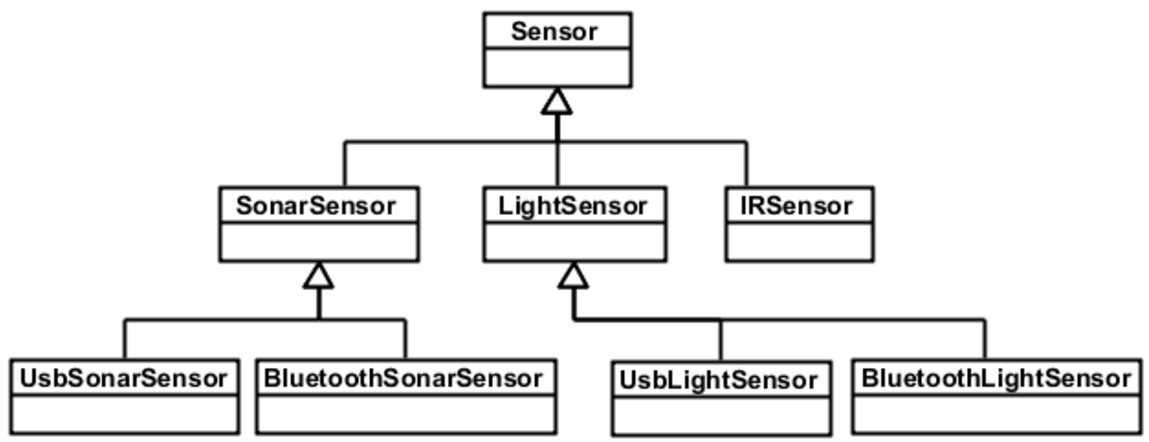
\includegraphics[width=0.7\textwidth]{noBridge.png}
			\Huge{$$\downarrow$$}
			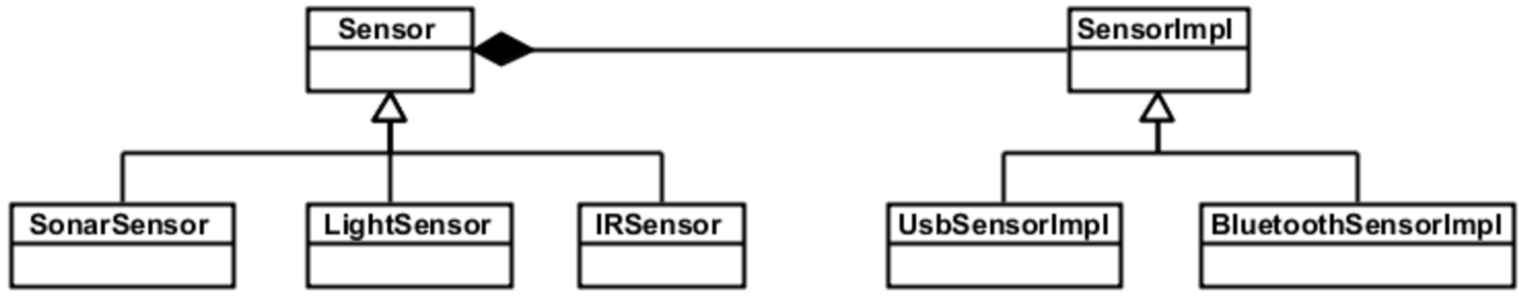
\includegraphics[width=0.7\textwidth]{bridge.png}
		\end{center}
	\end{frame}

	\begin{frame}
		\frametitle{``Мост'', общая схема}
		\begin{center}
			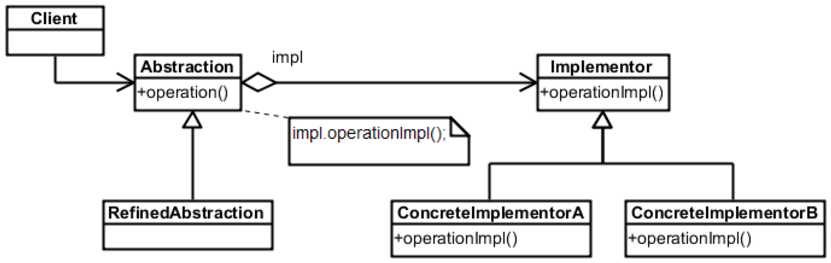
\includegraphics[width=0.7\textwidth]{bridgeGeneral.png}
		\end{center}
		\begin{itemize}
			\item \textit{Abstraction} --- определяет интерфейс абстракции, хранит ссылку на реализацию
			\item \textit{RefinedAbstraction} --- расширяет интерфейс абстракции, делает полезную работу, используя реализацию
			\item \textit{Implementor} --- определяет интерфейс реализации, в котором абстракции предоставляются низкоуровневые операции
			\item \textit{ConcreteImplementor} --- предоставляет конкретную реализацию Implementor
		\end{itemize}
	\end{frame}

	\begin{frame}
		\frametitle{Когда применять}
		\begin{itemize}
			\item Когда хочется разделить абстракцию и реализацию, например, когда реализацию можно выбирать во время компиляции или во время выполнения
			\begin{itemize}
				\item ``Стратегия'', ``Прокси''
			\end{itemize}
			\item Когда абстракция и реализация должны расширяться новыми подклассами
			\item Когда хочется разделить одну реализацию между несколькими объектами
			\begin{itemize}
				\item Как copy-on-write в строках
			\end{itemize}
		\end{itemize}
	\end{frame}

	\begin{frame}
		\frametitle{Тонкости реализации}
		Создание правильного Implementor-а
		\begin{itemize}
			\item Самой абстракцией в конструкторе, в зависимости от переданных параметров
			\begin{itemize}
				\item Как вариант --- выбор реализации по умолчанию и замена её по ходу работы
			\end{itemize}
			\item Принимать реализацию извне (как параметр конструктора, или, реже, как значение в сеттер)
			\item Фабрика/фабричный метод
			\begin{itemize}
				\item Позволяет спрятать платформозависимые реализации, чтобы не зависеть от них всех при сборке
			\end{itemize}
		\end{itemize}
	\end{frame}

	\begin{frame}
		\frametitle{Pointer To Implementation (PImpl)}
		Вырожденный мост для C++, когда ``абстракция'' имеет ровно одну реализацию, часто полностью дублирующую её интерфейс

		Зачем: чтобы клиенты класса не зависели при сборке от его реализации

		\begin{itemize}
			\item Позитивно сказывается на времени компиляции программ на C++
			\item Позволяет менять реализацию независимо
			\begin{itemize}
				\item Сохраняя бинарную совместимость
			\end{itemize}
		\end{itemize}

		Как: предварительное объявление класса-реализации, полное определение --- в .cpp-файле вместе с методами абстракции

		Часто используется в реализации библиотек (например, Qt)
	\end{frame}

	\begin{frame}
		\frametitle{Паттерн ``Приспособленец'' (Flyweight)}
		Предназначается для эффективной поддержки множества мелких объектов

		Пример:

		\begin{itemize}
			\item Есть текстовый редактор
			\item Хочется работать с каждым символом как с объектом
			\begin{itemize}
				\item Единообразие алгоритмов форматирования и внутренней структуры документа
				\item Более красивая и ООПшная реализация
				\begin{itemize}
					\item Паттерн ``Компоновщик'', структура ``Символ'' $\rightarrow$ ``Строка'' $\rightarrow$ ``Страница''
				\end{itemize}
			\end{itemize}
			\item Наивная реализация привела бы к чрезмерной расточительности по времени работы и по памяти, потому что документы с миллионами символов не редкость
		\end{itemize}
	\end{frame}

	\begin{frame}
		\frametitle{``Приспособленец'', пример}
		\begin{center}
			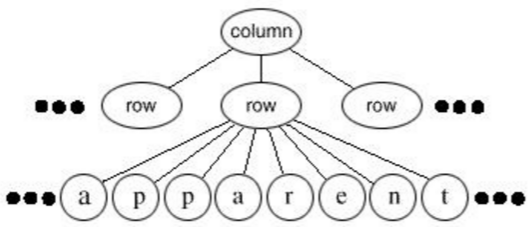
\includegraphics[width=0.38\textwidth]{noFlyweight.png}
			\raisebox{0.1\textheight}{\quad\Huge{$\rightarrow$}\quad}
			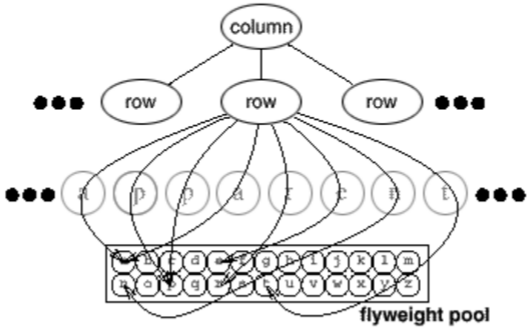
\includegraphics[width=0.38\textwidth]{flyweightExample.png}
		\end{center}
	\end{frame}

	\begin{frame}
		\frametitle{``Приспособленец'', общая схема}
		\begin{center}
			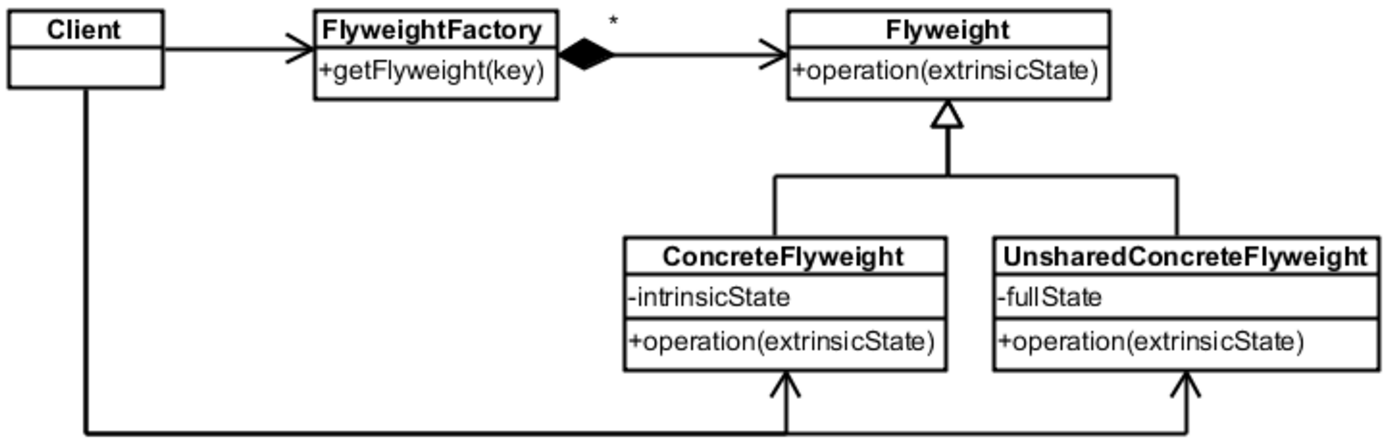
\includegraphics[width=0.7\textwidth]{flyweight.png}
		\end{center}
		\begin{footnotesize}
			\begin{itemize}
				\item \textit{Flyweight} --- определяет интерфейс, через который приспособленцы могут получать внешнее состояние
				\item \textit{ConcreteFlyweight} --- реализует интерфейс Flyweight и может иметь внутреннее состояние, не зависит от контекста
				\item \textit{UnsharedConcreteFlyweight} --- неразделяемый ``приспособленец'', хранящий всё состояние в себе, бывает нужен, чтобы собирать иерархические структуры из Flyweight-ов (``Компоновщик'')
				\item \textit{FlyweightFactory} --- содержит пул приспособленцев, создаёт их и управляет их жизнью
			\end{itemize}
		\end{footnotesize}
	\end{frame}

	\begin{frame}
		\frametitle{``Приспособленец'', диаграмма объектов}
		\begin{center}
			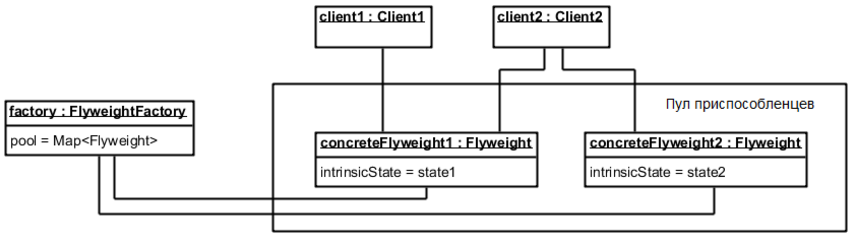
\includegraphics[width=0.7\textwidth]{flyweightObjects.png}
		\end{center}
		\begin{itemize}
			\item Клиенты могут быть разных типов
			\item Клиенты могут разделять приспособленцев
			\begin{itemize}
				\item Один клиент может иметь несколько ссылок на одного приспособленца
			\end{itemize}
			\item Во время выполнения клиенты имеют право не знать про фабрику
		\end{itemize}
	\end{frame}

	\begin{frame}
		\frametitle{Когда применять}
		\begin{itemize}
			\item Когда в приложении используется много мелких объектов
			\item Они допускают разделение состояния на внутреннее и внешнее
			\begin{itemize}
				\item Желательно, чтобы внешнее состояние было вычислимо
			\end{itemize}
			\item Идентичность объектов не важна
			\begin{itemize}
				\item Используется семантика Value Type
			\end{itemize}
			\item Главное, когда от такого разделения можно получить ощутимый выигрыш
		\end{itemize}
	\end{frame}

	\begin{frame}
		\frametitle{Тонкости реализации}
		\begin{itemize}
			\item Внешнее состояние --- по сути, отдельный объект, поэтому если различных внешних состояний столько же, сколько приспособленцев, смысла нет
			\begin{itemize}
				\item Один объект-состояние покрывает сразу несколько приспособленцев
				\begin{itemize}
					\item Например, объект ``Range'' может хранить параметры форматирования для всех букв внутри фрагмента
				\end{itemize}
			\end{itemize}
			\item Клиенты не должны инстанцировать приспособленцев сами, иначе трудно обеспечить разделение
			\begin{itemize}
				\item Имеет смысл иметь механизм для удаления неиспользуемых приспособленцев
				\begin{itemize}
					\item Если их может быть много
				\end{itemize}
			\end{itemize}
			\item Приспособленцы немутабельны и Value Objects (с правильно переопределённой операцией сравнения)
			\begin{itemize}
				\item Про hashCode() тоже надо не забыть
			\end{itemize}
		\end{itemize}
	\end{frame}

	\begin{frame}
		\frametitle{``Компоновщик'' (Composite), детали реализации}
		\begin{columns}
			\begin{column}{0.6\textwidth}
				\begin{itemize}
					\item Ссылка на родителя
					\begin{itemize}
						\item Может быть полезна для простоты обхода
						\item ``Цепочка обязанностей''
						\item Но дополнительный инвариант
						\item Обычно реализуется в Component
					\end{itemize}
				\end{itemize}
			\end{column}
			\begin{column}{0.4\textwidth}
				\begin{center}
					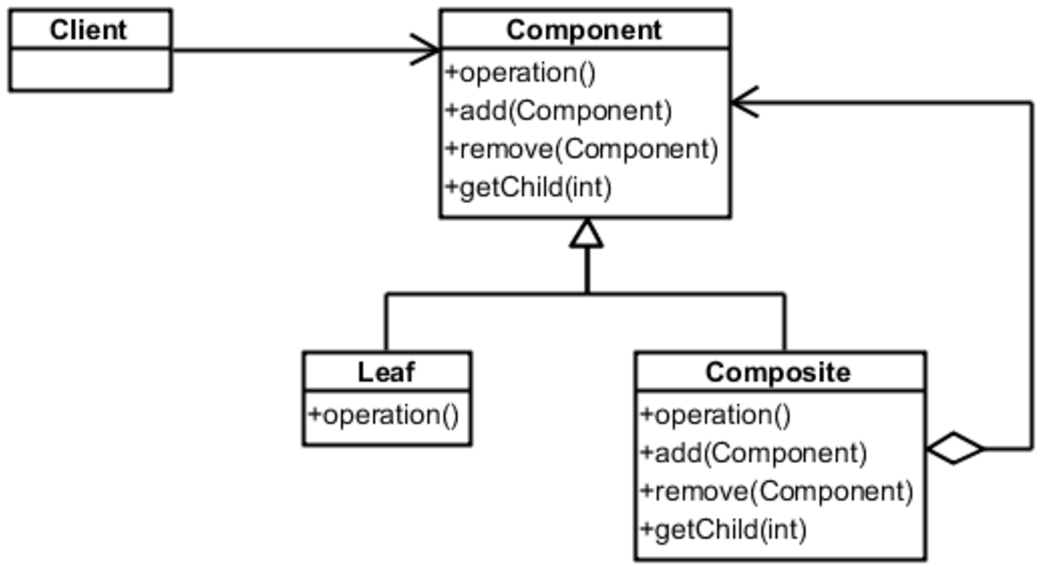
\includegraphics[width=\textwidth]{composite.png}
				\end{center}
			\end{column}
		\end{columns}

		\begin{itemize}
			\item Разделяемые поддеревья и листья
			\begin{itemize}
				\item Позволяют сильно экономить память
				\item Проблемы с навигацией к родителям и разделяемым состоянием
				\item Паттерн ``Приспособленец''
			\end{itemize}
			\item Идеологические проблемы с операциями для работы с потомками
			\begin{itemize}
				\item Не имеют смысла для листа
				\begin{itemize}
					\item Можно считать Leaf Composite-ом, у которого всегда 0 потомков
				\end{itemize}
				\item Операции add и remove можно объявить и в Composite, тогда придётся делать cast
				\begin{itemize}
					\item Иначе надо бросать исключения в add и remove
				\end{itemize}
			\end{itemize}
		\end{itemize}
	\end{frame}

	\begin{frame}
		\frametitle{``Компоновщик'', детали реализации (2)}
		\begin{itemize}
			\item Операция getComposite() – более аккуратный аналог cast-а
			\item Где определять список потомков
			\begin{itemize}
				\item В Composite, экономия памяти
				\item В Component, единообразие операций
				\item ``Список'' вполне может быть хеш-таблицей, деревом или чем угодно
			\end{itemize}
			\item Порядок потомков может быть важен, может нет
			\item Кеширование информации для обхода или поиска
			\begin{itemize}
				\item Например, кеширование ограничивающих прямоугольников для фрагментов картинки
				\item Инвалидация кеша
			\end{itemize}
			\item Удаление потомков
			\begin{itemize}
				\item Если нет сборки мусора, то лучше в Composite
				\item Следует опасаться разделяемых листьев/поддеревьев
			\end{itemize}
		\end{itemize}
	\end{frame}

	\begin{frame}
		\frametitle{``Декоратор'' (Decorator), детали реализации}
		\begin{columns}
			\begin{column}{0.6\textwidth}
				\begin{itemize}
					\item Интерфейс декоратора должен соответствовать интерфейсу декорируемого объекта
					\begin{itemize}
						\item Иначе получится ``Адаптер''
					\end{itemize}
					\item Если конкретный декоратор один, абстрактный класс можно не делать
				\end{itemize}
			\end{column}
			\begin{column}{0.4\textwidth}
				\begin{center}
					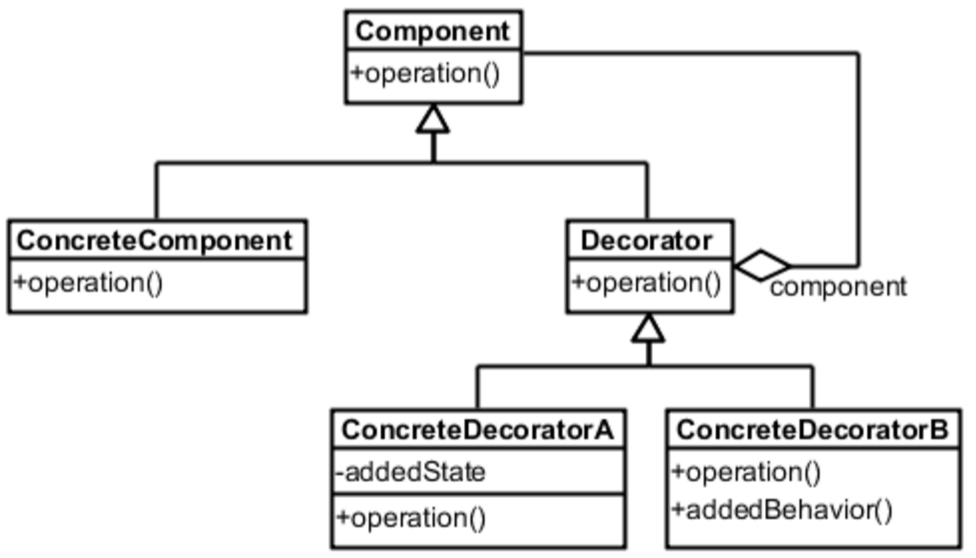
\includegraphics[width=\textwidth]{decorator.png}
				\end{center}
			\end{column}
		\end{columns}
		\begin{itemize}
			\item Component должен быть по возможности небольшим (в идеале, интерфейсом)
			\begin{itemize}
				\item Иначе лучше паттерн ``Стратегия''
				\item Или самодельный аналог, например, список ``расширений'', которые вызываются декорируемым объектом вручную перед операцией или после неё
			\end{itemize}
		\end{itemize}
	\end{frame}

	\begin{frame}
		\frametitle{``Стратегия'' (Strategy), детали реализации}
		\begin{center}
			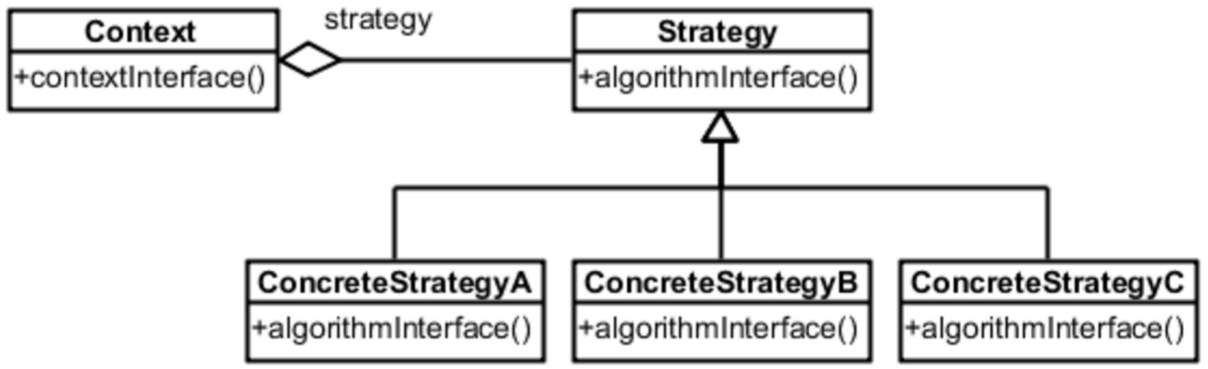
\includegraphics[width=0.6\textwidth]{strategy.png}
		\end{center}
		\begin{itemize}
			\item Передача контекста вычислений в стратегию
			\begin{itemize}
				\item Как параметры метода --- уменьшает связность, но некоторые параметры могут быть стратегии не нужны
				\item Передавать сам контекст в качестве аргумента --- в Context интерфейс для доступа к данным
			\end{itemize}
		\end{itemize}
	\end{frame}

	\begin{frame}
		\frametitle{``Стратегия'' (Strategy), детали реализации (2)}
		\begin{itemize}
			\item Стратегия может быть параметром шаблона
			\begin{itemize}
				\item Если не надо её менять на лету
				\item Не надо абстрактного класса и нет оверхеда на вызов виртуальных методов
			\end{itemize}
			\item Стратегия по умолчанию
			\begin{itemize}
				\item Или просто поведение по умолчанию, если стратегия не установлена
			\end{itemize}
			\item Объект-стратегия может быть приспособленцем
		\end{itemize}
	\end{frame}

	\begin{frame}
		\frametitle{``Адаптер'' (Adapter), детали реализации}
		\begin{columns}
			\begin{column}{0.5\textwidth}
				\begin{itemize}
					\item Адаптер объекта:
						\vspace{0.3cm}
						
						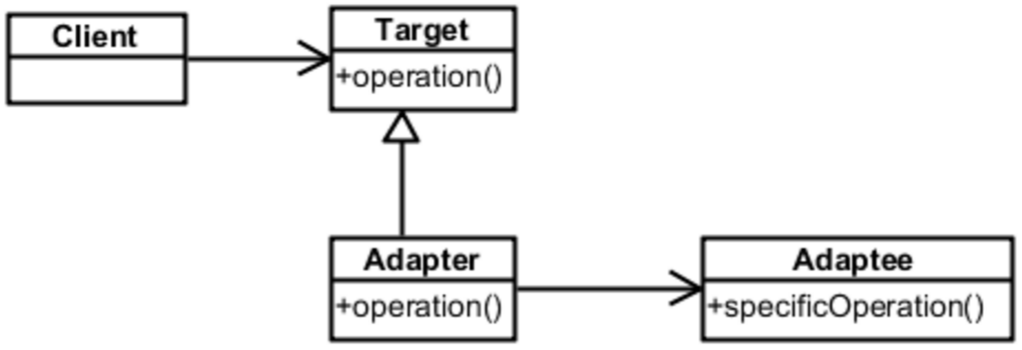
\includegraphics[width=0.8\textwidth]{objectAdapter.png}
						\vspace{0.3cm}
					\item Похоже на ``Мост''
				\end{itemize}
			\end{column}
			\begin{column}{0.5\textwidth}
				\begin{itemize}
					\item Адаптер класса:
						\vspace{0.3cm}
						
						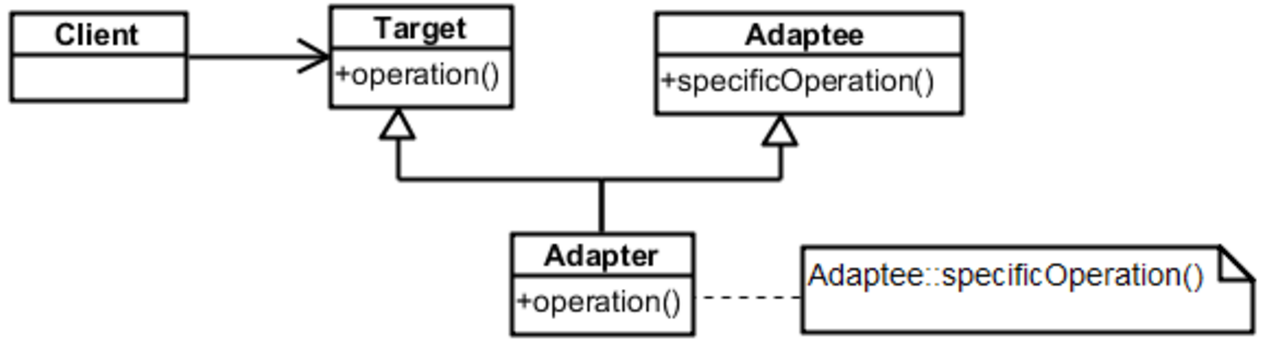
\includegraphics[width=0.9\textwidth]{classAdapter.png}
						\vspace{0.3cm}
					\item Нужно множественное наследование
					\begin{itemize}
						\item private-наследование в C++
					\end{itemize}
				\end{itemize}
			\end{column}
		\end{columns}
	\end{frame}

	\begin{frame}
		\frametitle{``Заместитель'' (Proxy), детали реализации}
		\begin{center}
			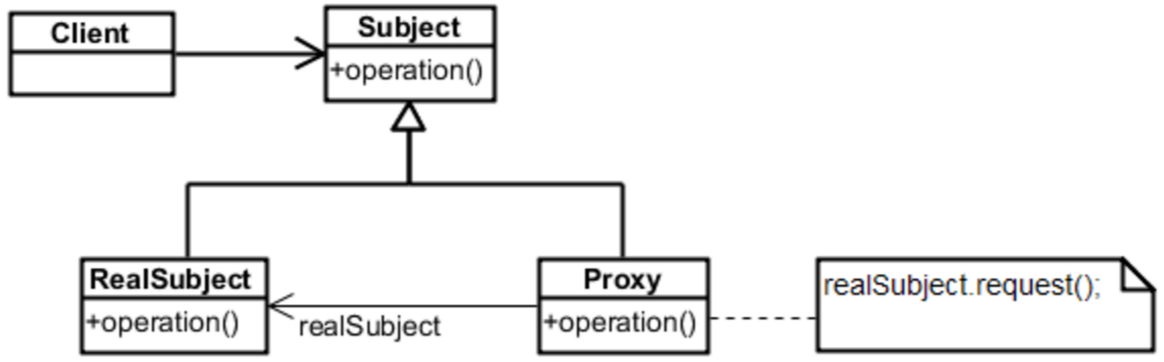
\includegraphics[width=0.7\textwidth]{proxy.png}
		\end{center}
		\begin{itemize}
			\item Перегрузка оператора доступа к членам класса (для C++)
			\begin{itemize}
				\item Умные указатели так устроены
				\item C++ вызывает операторы \mintinline{c++}|->| по цепочке
				\begin{itemize}
					\item \mintinline{c++}|object->do()| может быть хоть \mintinline{c++}|((object.operator->()).operator->()).do()|
				\end{itemize}
				\item Не подходит, если надо различать операции
			\end{itemize}
		\end{itemize}
	\end{frame}

	\begin{frame}
		\frametitle{``Заместитель'' (Proxy), детали реализации (2)}
		\begin{itemize}
			\item Реализация ``вручную'' всех методов проксируемого объекта
			\begin{itemize}
				\item Сотня методов по одной строчке каждый
				\item C\#/F\#: \mintinline{csharp}|public void do() => realSubject.do();|
				\item Препроцессор/генерация
				\begin{itemize}
					\item Технологии наподобие WCF
				\end{itemize}
			\end{itemize}
			\item Проксируемого объекта может не быть в памяти
		\end{itemize}
	\end{frame}

	\begin{frame}
		\frametitle{``Фасад'' (Facade), детали реализации}
		\begin{columns}
			\begin{column}{0.5\textwidth}
				\begin{itemize}
					\item Абстрактный Facade
					\begin{itemize}
						\item Существенно снижает связность клиента с подсистемой
					\end{itemize}
				\end{itemize}
			\end{column}
			\begin{column}{0.5\textwidth}
				\begin{center}
					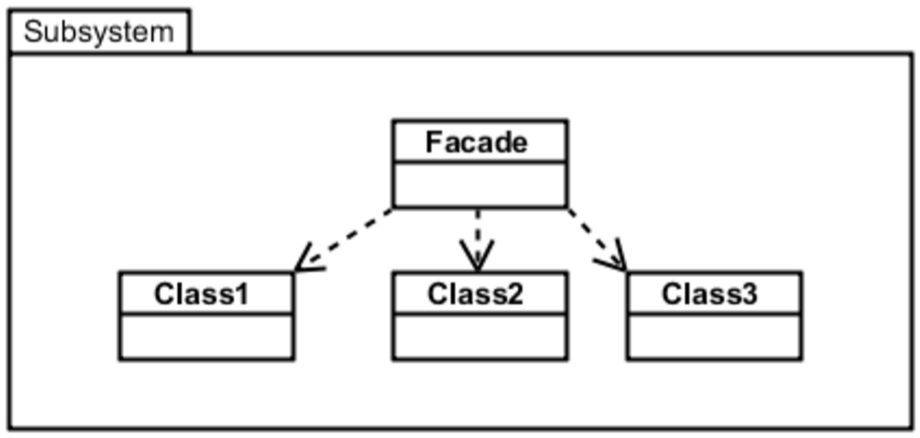
\includegraphics[width=0.8\textwidth]{facade.png}
				\end{center}
			\end{column}
		\end{columns}
		\begin{itemize}
			\item Открытые и закрытые классы подсистемы
			\begin{itemize}
				\item Пространства имён и пакеты помогают, но требуют дополнительных соглашений
				\begin{itemize}
					\item Пространство имён details
				\end{itemize}
				\item Инкапсуляция целой подсистемы --- это хорошо
			\end{itemize}
		\end{itemize}
	\end{frame}

	\section{Порождающие шаблоны}

	\begin{frame}
		\frametitle{``Фабричный метод'' (Factory Method), детали реализации}
		\begin{center}
			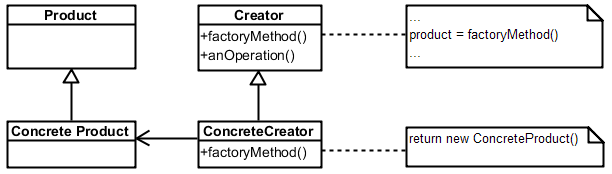
\includegraphics[width=0.6\textwidth]{factoryMethod.png}
		\end{center}
		\begin{itemize}
			\item Абстрактный Creator или реализация по умолчанию
			\begin{itemize}
				\item Второй вариант может быть полезен для расширяемости
			\end{itemize}
			\item Параметризованные фабричные методы
			\item Если язык поддерживает инстанциацию по прототипу (JavaScript, Smalltalk), можно хранить порождаемый объект
			\item Creator не может вызывать фабричный метод в конструкторе
			\item Можно сделать шаблонный Creator
		\end{itemize}
	\end{frame}

	\begin{frame}
		\frametitle{``Абстрактная фабрика'' (Abstract Factory), детали реализации}
		\begin{columns}
			\begin{column}{0.5\textwidth}
				\begin{itemize}
					\item Хорошо комбинируются с паттерном ``Одиночка''
					\item Если семейств продуктов много, то фабрика может инициализироваться \textit{прототипами}, тогда не надо создавать сотню подклассов
				\end{itemize}
			\end{column}
			\begin{column}{0.5\textwidth}
				\begin{center}
					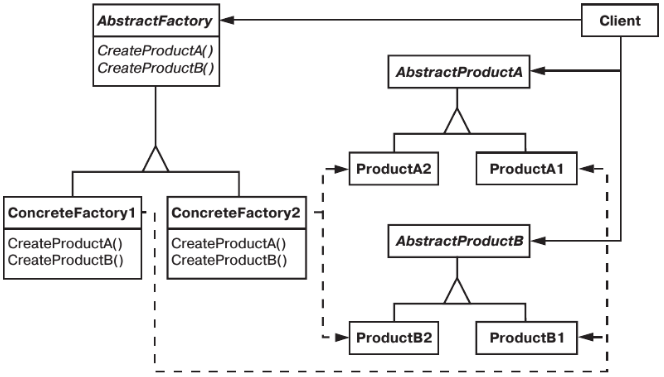
\includegraphics[width=\textwidth]{abstractFactory.png}
				\end{center}
			\end{column}
		\end{columns}
		\begin{itemize}
			\item Прототип на самом деле может быть классом (например, Class в Java)
			\item Если виды объектов часто меняются, может помочь параметризация метода создания
			\begin{itemize}
				\item Может пострадать типобезопасность
			\end{itemize}
		\end{itemize}
	\end{frame}

	\begin{frame}
		\frametitle{``Прототип'' (Prototype), детали реализации}
		\begin{columns}
			\begin{column}{0.45\textwidth}
				\begin{itemize}
					\item Паттерн интересен только для языков, где мало runtime-информации о типе (C++)
					\item Реестр прототипов, обычно ассоциативное хранилище
				\end{itemize}
			\end{column}
			\begin{column}{0.55\textwidth}
				\begin{center}
					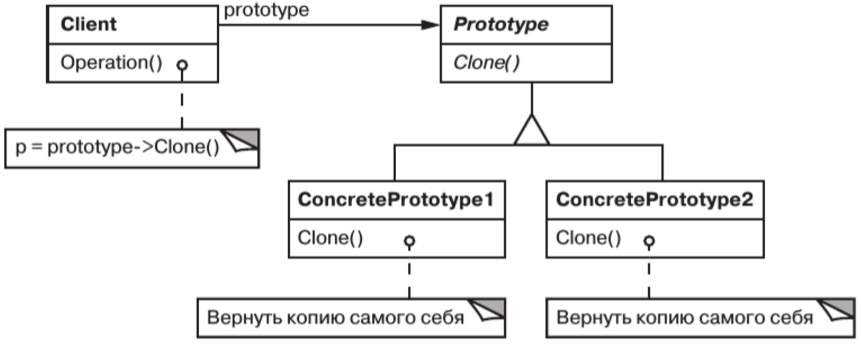
\includegraphics[width=\textwidth]{prototype.png}
				\end{center}
			\end{column}
		\end{columns}
		\begin{itemize}
			\item Операция Clone
			\begin{itemize}
				\item Глубокое и мелкое копирование
				\item В случае, если могут быть круговые ссылки
				\item Сериализовать/десериализовать объект (но помнить про идентичность)
			\end{itemize}
			\item Инициализация клона
			\begin{itemize}
				\item Передавать параметры в Clone --- плохая идея
			\end{itemize}
		\end{itemize}
	\end{frame}

	\begin{frame}
		\frametitle{``Строитель'' (Builder), детали реализации}
		\begin{center}
			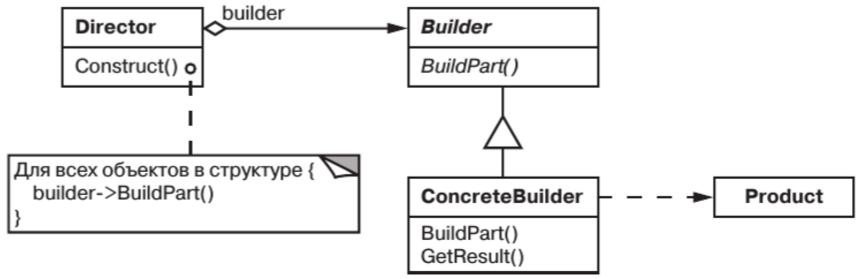
\includegraphics[width=0.7\textwidth]{builder.png}
		\end{center}
		\begin{itemize}
			\item Абстрактные и конкретные строители
			\begin{itemize}
				\item Достаточно общий интерфейс
			\end{itemize}
			\item Общий интерфейс для продуктов не требуется
			\begin{itemize}
				\item Клиент конфигурирует распорядителя конкретным строителем, он же и забирает результат
			\end{itemize}
			\item Пустые методы по умолчанию
		\end{itemize}
	\end{frame}

	\begin{frame}[fragile]
		\frametitle{``Строитель'', примеры}
		\begin{itemize}
			\item StringBuilder
			\item Guava, подсистема работы с графами
			\begin{minted}{java}
MutableNetwork<Webpage, Link> webSnapshot = 
        NetworkBuilder.directed()
    .allowsParallelEdges(true)
    .nodeOrder(ElementOrder.natural())
    .expectedNodeCount(100000)
    .expectedEdgeCount(1000000)
    .build();
			\end{minted}
		\end{itemize}
	\end{frame}

	\section{Поведенческие шаблоны}

	\begin{frame}
		\frametitle{``Шаблонный метод'' (Template Method), детали реализации}
		\begin{columns}
			\begin{column}{0.5\textwidth}
				\begin{itemize}
					\item Сам шаблонный метод, как правило, невиртуальный
					\item Лучше использовать соглашения об именовании, например, называть операции с Do
				\end{itemize}
			\end{column}
			\begin{column}{0.4\textwidth}
				\begin{center}
					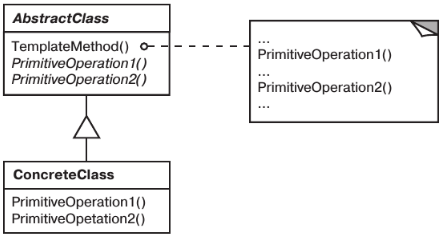
\includegraphics[width=\textwidth]{templateMethod.png}
				\end{center}
			\end{column}
		\end{columns}
		\begin{itemize}
			\item Примитивные операции могут быть виртуальными или чисто виртуальными
			\begin{itemize}
				\item Лучше их делать protected
				\item Чем их меньше, тем лучше
			\end{itemize}
		\end{itemize}
	\end{frame}

	\begin{frame}
		\frametitle{``Посредник'' (Mediator), детали реализации}
		\begin{columns}
			\begin{column}{0.5\textwidth}
				\begin{itemize}
					\item Абстрактный класс ``Mediator'' часто не нужен
					\item Паттерн ``Наблюдатель'': медиатор подписывается на события в коллегах
					\item Наоборот: коллеги вызывают методы медиатора
				\end{itemize}
			\end{column}
			\begin{column}{0.5\textwidth}
				\begin{center}
					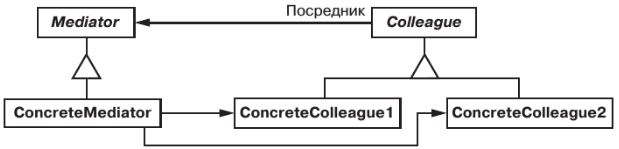
\includegraphics[width=\textwidth]{mediatorClasses.png}
					\vspace{1cm}
					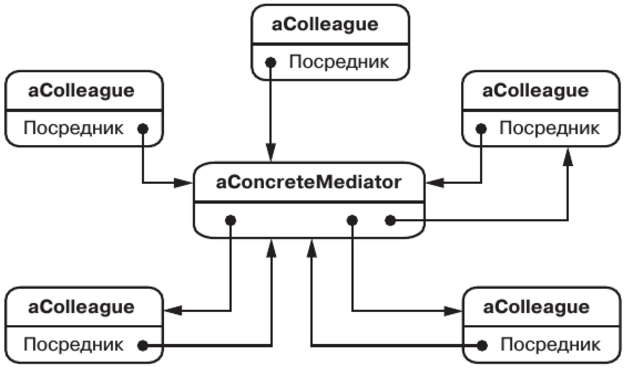
\includegraphics[width=\textwidth]{mediatorObjects.png}
				\end{center}
			\end{column}
		\end{columns}
	\end{frame}

	\begin{frame}
		\frametitle{``Команда'' (Command), детали реализации}
		\begin{center}
			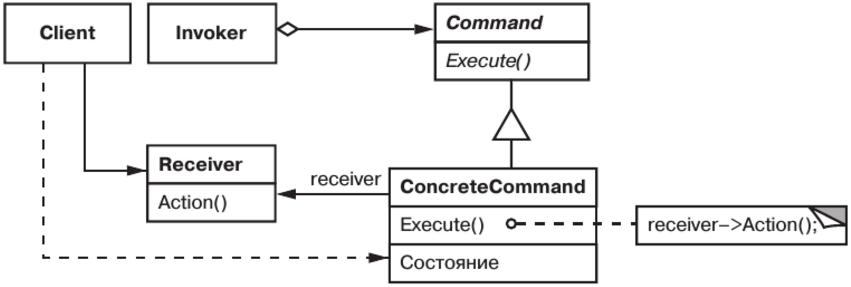
\includegraphics[width=0.6\textwidth]{command.png}
		\end{center}
		\begin{itemize}
			\item Насколько ``умной'' должна быть команда
			\item Отмена и повторение операций --- тоже от хранения всего состояния в команде до ``вычислимого'' отката
			\begin{itemize}
				\item Undo-стек и Redo-стек
				\item Может потребоваться копировать команды
				\item ``Искусственные'' команды
				\item Композитные команды
			\end{itemize}
			\item Паттерн ``Хранитель'' для избежания ошибок восстановления
		\end{itemize}
	\end{frame}

	\begin{frame}[fragile]
		\frametitle{``Команда'', пример}
		\begin{itemize}
			\item Qt, класс QAction:
			\begin{minted}{c++}
const QIcon openIcon = QIcon(":/images/open.png");
QAction *openAct = new QAction(openIcon, tr("&Open..."), this);

openAct->setShortcuts(QKeySequence::Open);
openAct->setStatusTip(tr("Open an existing file"));

connect(openAct, &QAction::triggered, this, &MainWindow::open);

fileMenu->addAction(openAct);
fileToolBar->addAction(openAct);
			\end{minted}
		\end{itemize}
	\end{frame}

	\begin{frame}
		\frametitle{``Цепочка ответственности'' (Chain of Responsibility), детали реализации}
		\begin{columns}
			\begin{column}{0.5\textwidth}
				\begin{itemize}
					\item Необязательно реализовывать связи в цепочке специально
					\begin{itemize}
						\item На самом деле, чаще используются существующие связи
					\end{itemize}

				\end{itemize}
			\end{column}
			\begin{column}{0.5\textwidth}
				\begin{center}
					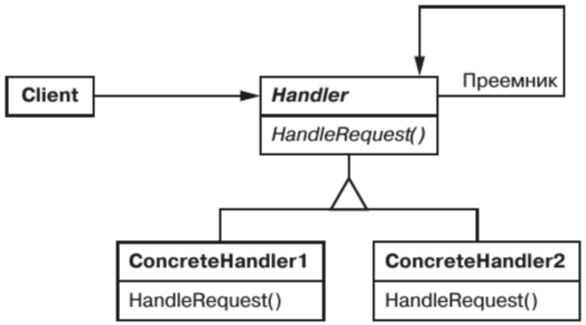
\includegraphics[width=\textwidth]{chainOfResponsibility.png}
				\end{center}
			\end{column}
		\end{columns}
		\begin{itemize}
			\item По умолчанию в Handler передавать запрос дальше (если ссылки на преемника всё-таки есть)
			\item Если возможных запросов несколько, их надо как-то различать
			\begin{itemize}
				\item Явно вызывать методы --- нерасширяемо
				\item Использовать объекты-запросы
			\end{itemize}
		\end{itemize}
	\end{frame}

	\begin{frame}[fragile]
		\frametitle{``Цепочка ответственности'', примеры}
		\begin{itemize}
			\item Распространение исключений
			\item Распространение событий в оконных библиотеках:
			\begin{minted}{c++}
void MyCheckBox::mousePressEvent(QMouseEvent *event)
{
    if (event->button() == Qt::LeftButton) {
        // handle left mouse button here
    } else {
        // pass on other buttons to base class
        QCheckBox::mousePressEvent(event);
    }
}
			\end{minted}
		\end{itemize}
	\end{frame}

	\begin{frame}
		\frametitle{``Наблюдатель'' (Observer), детали реализации}
		\begin{itemize}
			\item В ``нормальных'' языках поддержан ``из коробки'' (через механизм событий)
		\end{itemize}
		\begin{columns}
			\begin{column}{0.45\textwidth}
				\begin{itemize}
					\item Могут использоваться хеш-таблицы для отображения субъектов и наблюдателей
					\begin{itemize}
						\item Так делает WPF в .NET, есть даже языковая поддержка в C\#
					\end{itemize}
				\end{itemize}
			\end{column}
			\begin{column}{0.55\textwidth}
				\begin{center}
					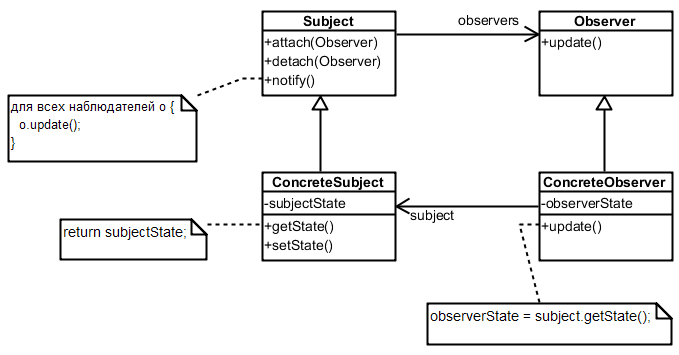
\includegraphics[width=\textwidth]{observer.png}
				\end{center}
			\end{column}
		\end{columns}
		\begin{itemize}
			\item Необходимость идентифицировать субъект
			\item Кто инициирует нотификацию
			\begin{itemize}
				\item Операции, модифицирующие субъект
				\item Клиент, после серии модификаций субъекта
			\end{itemize}
		\end{itemize}
	\end{frame}

	\begin{frame}
		\frametitle{``Наблюдатель'' (Observer), детали реализации (2)}
		\begin{itemize}
			\item Ссылки на субъектов и наблюдателей
			\begin{itemize}
				\item Простой способ организовать утечку памяти в C\# или грохнуть программу в C++
			\end{itemize}
			\item Консистентность субъекта при отправке нотификации
			\begin{itemize}
				\item Очевидно, но легко нарушить, вызвав метод предка в потомке
				\item ``Шаблонный метод''
				\item Документировать, кто когда какие события бросает
			\end{itemize}
			\item Передача сути изменений --- pull vs push
			\item Фильтрация по типам событий
			\item Менеджер изменений (``Посредник'')
		\end{itemize}
	\end{frame}

	\begin{frame}[fragile]
		\frametitle{``Наблюдатель'', пример (1)}
		\begin{itemize}
			\item События в C\#:
			\begin{minted}{csharp}
internal class NewMessageEventArgs : EventArgs {
    private readonly string message;
    public MessageEventArgs(string message) 
        => this.message = message;
    public string Message => message;
}
			\end{minted}
		\end{itemize}
	\end{frame}

	\begin{frame}[fragile]
		\frametitle{``Наблюдатель'', пример (2)}
		\begin{small}
			\begin{minted}{csharp}
internal class Messenger {
    public event EventHandler<NewMessageEventArgs> NewMessage;
    protected virtual void OnMessage(NewMessageEventArgs e) {
        EventHandler<NewMessageEventArgs> temp 
                = Volatile.Read(ref NewMessage);
        if (temp != null) 
            temp(this, e);
    }
    public void SimulateMessage(String message) {
        NewMessageEventArgs e = new NewMessageEventArgs(message);
        OnMessage(e);
    }
}
			\end{minted}
		\end{small}
	\end{frame}

	\begin{frame}[fragile]
		\frametitle{``Наблюдатель'', пример (3)}
		\begin{itemize}
			\begin{minted}{csharp}
internal sealed class Fax {
    public Fax(Messenger mm) => mm.NewMessage += FaxMsg;

    private void FaxMsg(object sender, NewMessageEventArgs e) {
        Console.WriteLine("Faxing message:");
        Console.WriteLine($"Message={e.Message}");
    }

    public void Unregister(Messenger mm) 
            => mm.NewMessage -= FaxMsg;
}
			\end{minted}
		\end{itemize}
	\end{frame}

	\begin{frame}
		\frametitle{``Состояние'' (State), детали реализации}
		\begin{columns}
			\begin{column}{0.5\textwidth}
				\begin{itemize}
					\item Переходы между состояниями --- в Context или в State?
					\item Таблица переходов
					\begin{itemize}
						\item Трудно добавить действия по переходу
					\end{itemize}
				\end{itemize}
			\end{column}
			\begin{column}{0.5\textwidth}
				\begin{center}
					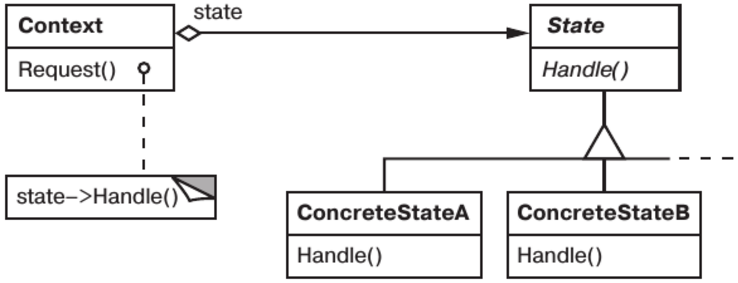
\includegraphics[width=\textwidth]{state.png}
				\end{center}
			\end{column}
		\end{columns}
		\begin{itemize}
			\item Создание и уничтожение состояний
			\begin{itemize}
				\item Создать раз и навсегда
				\item Создавать и удалять при переходах
			\end{itemize}
		\end{itemize}
	\end{frame}

	\begin{frame}
		\frametitle{``Посетитель'' (Visitor), детали реализации}
		\begin{columns}
			\begin{column}{0.4\textwidth}
				\begin{itemize}
					\item Использовать перегрузку методов Visit(...)
					\item Чаще всего сама коллекция отвечает за обход, но может быть итератор
					\item Может даже сам Visitor, если обход зависит от результата операции
				\end{itemize}
			\end{column}
			\begin{column}{0.6\textwidth}
				\begin{center}
					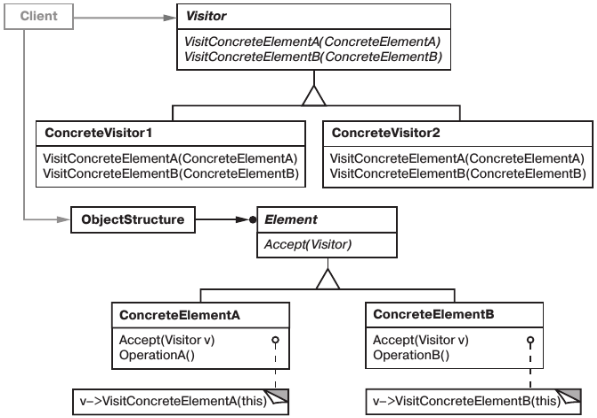
\includegraphics[width=\textwidth]{visitor.png}
				\end{center}
			\end{column}
		\end{columns}
	\end{frame}

% 	\begin{frame}[fragile]
% 		\frametitle{``Посетитель'', пример}
% 		\begin{itemize}
% 			\begin{minted}{csharp}
% 				Здесь будет пример кода на ANTLR
% 			\end{minted}
% 		\end{itemize}
% \end{frame}

	\begin{frame}
		\frametitle{``Хранитель'' (Memento), детали реализации}
		\begin{center}
			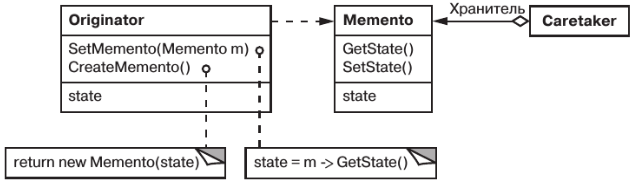
\includegraphics[width=0.7\textwidth]{memento.png}
		\end{center}
		\begin{itemize}
			\item Два интерфейса: ``широкий'' для хозяев и ``узкий'' для остальных объектов
			\begin{itemize}
				\item Требуется языковая поддержка
			\end{itemize}
			\item Можно хранить только дельты состояний
		\end{itemize}
	\end{frame}

	\begin{frame}
		\frametitle{``Интерпретатор'' (Interpreter)}
		Определяет представление грамматики и интерпретатор для заданного языка.
		\begin{center}
			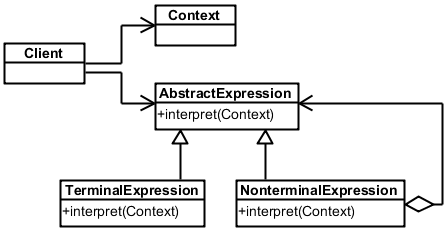
\includegraphics[width=0.6\textwidth]{interpreter.png}
		\end{center}
		\begin{itemize}
			\item Грамматика должна быть проста (иначе лучше ``Visitor'')
			\item Эффективность не критична
		\end{itemize}
	\end{frame}

	\begin{frame}
		\frametitle{``Интерпретатор'', пример}
		\begin{center}
			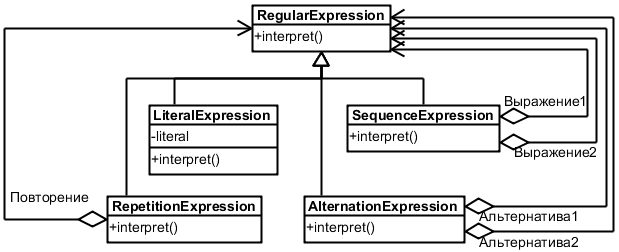
\includegraphics[width=0.8\textwidth]{regexp.png}
		\end{center}
	\end{frame}

	\begin{frame}
		\frametitle{``Интерпретатор'', детали реализации}
		\begin{footnotesize}
			\textbf{10-е правило Гринспена:}
			
			\textit{Любая достаточно сложная программа на Си или Фортране содержит заново написанную, неспецифицированную, глючную и медленную реализацию половины языка Common Lisp}
		\end{footnotesize}
		\begin{itemize}
			\item Построение дерева --- отдельная задача
			\item Несколько разных операций над деревом --- лучше ``Visitor''
			\item Можно использовать ``Приспособленец'' для разделения терминальных символов
		\end{itemize}
	\end{frame}

	\begin{frame}
		\frametitle{``Итератор'' (Iterator)}
		Инкапсулирует способ обхода коллекции.
		\begin{center}
			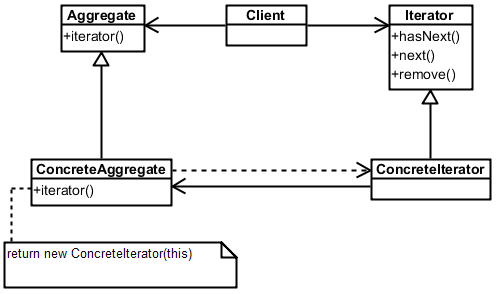
\includegraphics[width=0.6\textwidth]{iterator.png}
		\end{center}
		\begin{itemize}
			\item Разные итераторы для разных способов обхода
			\item Можно обходить не только коллекции
		\end{itemize}
	\end{frame}

	\begin{frame}[fragile]
		\frametitle{``Итератор'', примеры}
		\begin{itemize}
			\item Java-стиль:
			\begin{minted}{java}
public interface Iterator<E> {
    boolean hasNext();
    E next();
    void remove();
}
			\end{minted}
			\item .NET-стиль:
			\begin{minted}{csharp}
public interface IEnumerator<T>
{
    bool MoveNext();
    T Current { get; }
    void Reset();
}
			\end{minted}
		\end{itemize}
	\end{frame}

	\begin{frame}[fragile]
		\frametitle{``Итератор'', детали реализации (1)}
		\begin{itemize}
			\item Внешние итераторы
			\begin{minted}{csharp}
foreach (Thing t in collection)
{
    Console.WriteLine(t);
} 
			\end{minted}
			\item Внутренние итераторы
			\begin{minted}{csharp}
collection.ToList().ForEach(t => Console.WriteLine(t));
			\end{minted}
		\end{itemize}
	\end{frame}

	\begin{frame}
		\frametitle{``Итератор'', детали реализации (2)}
		\begin{itemize}
			\item Итераторы и курсоры
			\item Устойчивые и неустойчивые итераторы
			\begin{itemize}
				\item Паттерн ``Наблюдатель''
				\item Даже обнаружение модификации коллекции может быть непросто
			\end{itemize}
			\item Дополнительные операции
			\item В C++ итераторы --- это сложно
		\end{itemize}
	\end{frame}

\end{document}